\chapter{Evaluation des Trainings durch Probanden}
Mit der Evaluation wird die Auswertung der empirischen Methode zur Erfassung der Interaktionen mit dem Sofa erläutert. Weiterhin möchte der Autor die Ergebnisse und Erkenntnisse des neuronalen Netzes und des Gesamtsystems zeigen. Zudem finden in den folgenden Kapiteln auch die Beschreibungen des Aufbaus vom Prototypen auf einem realen Sofa statt. Der Autor möchte also eine Zusammenfassung der Ergebnisse und der empirischen Methode veranschaulichen, um daraus in Teil Sechs der Bachelorarbeit ein Fazit zu ziehen.

\section{Umgebung zur Erkennung von Interaktionen}
\label{sec:er_in}
Der Prototyp ist so aufgebaut, dass er beliebig um Sitzflächen auf einem Sofa erweitert werden kann. Für die empirische Methode wurde sich dafür entschieden, die Anzahl auf drei Sitzplätze zu beschränken. So kann das Sofa aus Abbildung \ref{fig:prot} benutzt werden. Jede zusammengesetzte Komponente aus Sensoren am ESP32 steht für einen Platz auf dem Sofa. Zwei ESPs haben einen FSR-Sensor mehr, da diese an den äußeren Sitzplätzen mit einer Armlehne ausgestattet sind. Für den akutellen Prototypen ist es nicht wichtig in welchem Raum, welche Möbel zusätzlich und welche Geräte vorhanden sind. Außerdem gibt es zwei unterschiedlich große FSR-Sensoren, die die gleichen Messwerte liefern und somit keine unterschiedliche Auswirkung auf die Sensorwerte im Datensatz haben.
\newline
\begin{figure}[H]
	\centering
		%[natürliche Breite in Pixeln, natürliche Höhe in Pixeln, Abhängigkeit von der Textbreite]
		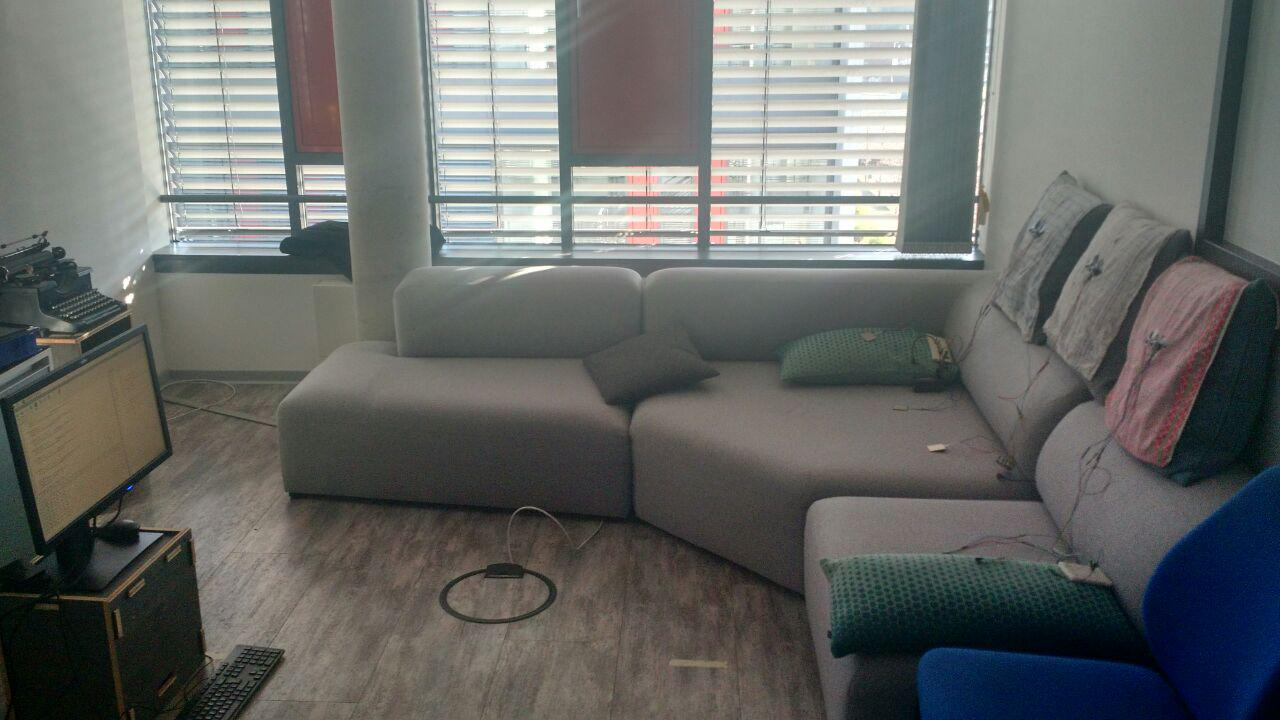
\includegraphics[width=0.75\textwidth]{images/prototyp.jpg}
	\caption{Realer Aufbau des Prototyps}
	\label{fig:prot}
\end{figure}

Abbildung \ref{fig:prot} zeigt den Prototypen, welcher auf einem Sofa aufgebaut ist. Die beiden grünen äußeren Kissen stellen die Armlehnen dar. Das wird gemacht, da dieses Sofa keine Armlehnen angebaut hat. Da der Prototyp für ein drei Personen Sofa ausgelegt ist, werden die Sitzplätze durch drei oben liegende Kissen getrennt. Auf der linken Seite ist der Raspberry Pi, mit dem darauf ausgeführten MQTT-Broker und Python-Programm zur Erfassung der Sensorwerte. Die Abbildung macht sichtbar, dass die Verwendung von Ultrasonic-Sensoren nicht positiv ist. Man kann also zum Schluss kommen, dass statt Ultrasonic-Sensoren, dünnere Sensoren die weniger auffallen, eingebaut werden müssen. Wenn Ultrasonic-Sensoren verwendet werdeb, dann muss immer eine Fläche in den Sofalehnen zusätzlich frei sein. Der Sensor kann dann dementsprechend den Abstand messen und der Nutzer muss sich immer im Radius der Wellen zur Messung des Abstands an die Rückenlehne anlehnen. Eine Möglichkeit zur Lösung des Problems kann durch Austauschen der Ultrasonic-Sensoren erfolgen, indem Sensoren verwendet werden, welche mehr Platz von der Rückenlehen einnehmen. Alternativ können mehrere kleine Sensoren verwendet werden.

\section{Soll-Ablauf der Situation}
\label{sec:abl}
Dieses Kapitel befasst sich mit der Beschreibung eines Ablaufs zur Sammlung der Daten indem die Probanden mit dem Sofa interagieren. Die folgende Beschreibung der Vorgehensweise zeigt, wie ein Proband in der Theorie mit dem Sofa interagiert, um die bestmögliche Erfassung der Sensordaten zu bekommen.
\newline
\newline
Um die Klassifizierung richtig vorhersehen zu können, erstellen Probanden durch Interaktionen mit Sofa einen Datensatz für die Trainings- und die Testphase wie sie in Kapitel \ref{subsec:eval} beschrieben ist. Ein Proband befindet sich immer alleine im Raum mit dem Sofa. So kann kein anderer Proband durch seine Interaktionen beeinflusst werden. Dort nimmt er verschiedene Positionen auf dem Sofa ein. Hat dieser seine Position festgelegt, werden die Sensorwerte in die CSV-Datei hinzugefügt. Die Position muss immer eine andere sein, damit die Variation mit den Sensoren sich so oft wie möglich unterscheidet. Der Proband soll sich immer hinlegen, hinsetzen oder das Sofa leer lassen. Der Ablauf ist mit jedem Probanden gleich und unterscheidet sich nur von den Interaktionen auf dem Sofa. Sobald 12 bis 15 Probanden diese Situation absolviert haben, wird das neuronale Netz mit diesem Datensatz trainiert und angepasst.
Die Probanden sehen außerdem auf dem Monitor, welche Position sie eingenommen haben in Form von den Sensordaten durch die Sensoren die sie benutzen.
\newline
Durch das Sammeln der Daten für den Datensatz soll außerdem getestet werden, wie die Probanden mit dem Sofaprotoypen umgehen und wie diese damit zurechtkommen. So wird dann gezeigt, welche Änderungen an dem Prototypen vorgenommen werden müssen, damit die Probanden die bestmögliche Interaktion mit dem Sofa ausführen können.

\newpage

\section{Tatsächlicher Ablauf aller Probanden}
\label{sub:real}
Der Autor führt aus Kapitel \ref{sec:abl} an, wie eine Datensammlung in der Theorie mit einem Probanden ablaufen soll. Der tatsächliche Ablauf mit allen Probanden erweist sich aber als Differenz zur Theorie. Insgesamt wurden mit 17 Probanden Daten gesammelt. In manchen fällen befanden sich mehrere Probanden im Raum, was den Interaktionen geholfen hat. Denn nicht jeder Proband kann sich sofort vorstellen, was mit den Interaktionen auf dem Sofa gemeint ist.
\newline
Jeder Proband nimmt verschiedene Positionen ein und auch unterschiedlich viele, da verschiedene Interaktionen mehrfach auftreten. Je mehr Probanden mit dem Sofa interagieren, desto häufiger treten damit die gleichen Positionen auf. Die Anzahl an Positionen nimmt mit mehr Probanden über die Zeit ab. Damit alle Probanden die gleiche Situation haben, ändert sich der Raum und das Sofa nicht. So hat jeder Proband die gleichen Voraussetzungen. Für diese empirische Methode ist auch kein smartes Gerät oder Möbelstück vorhanden. Da hier nur Sensordaten erfasst werden und das neuronale Netz noch keine entsprechende Vorhersage machen kann die immer korrekt ist.
\newline
Teile des Prototyps müssen zwischen den Interaktionen der Probanden auch hin und wieder neu zusammen gebaut werden, da es passieren kann, dass beim Anlehnen an die jeweilige Rückenlehne ein Kabel von den Ultrasonic-Sensoren durch den Probanden ohne Absicht getrennt wird. Die FSR-Sensoren sind zum Großteil nicht davon betroffen, da die Interaktionen nicht so stark auf die Kabel einwirken wie bei den Ultrasonic-Sensoren. Abgesehen davon gibt es mit den Interaktionen keine weiteren Probleme, außer das nicht jeder Proband immer selbstständig weiß, welche Positionen er machen muss. Dies ist aber unwichtig, da es bei dieser Datensammlung auch darum geht zu Testen, welche Änderungen am Prototyp gemacht werden müssen, damit der Proband besser mit dem System zurecht kommt.

\section{Aufbau des Datensatzes}
\label{sec:dataset}
In diesem Kapitel soll gezeigt werden, wie die Sensordaten für die Trainings- und Testphase gespeichert werden. Eine Position des Probanden ist eine Liste, die als eine Zeile in einer CSV-Datei liegt. Eine weitere CSV-Datei enthält die Positionen, die dem neuronalen Netz mit eingegeben werden. Kapitel \ref{subsec:ergeb} diskutiert die Ergebnisse aus dem neuronalen Netz und welche Optimierungen im weiteren vorgenommen werden, um die Vorhersagen mit den Testdaten genauer darzustellen. Die Tabelle \ref{tab:tablearr} stellt in abwärtiger Reihenfolge die festen Positionen der Sensoren in einem Array dar. Das folgende Beispiel der Daten einer CSV-Datei, zeigt die Positionen als Beispiel.
\newpage
\[0, 0, 134, 0, 3095, 0, 0, 717\]  
\[4095, 4095, 426, 84, 417, 580, 41, 456\]
\[0, 718, 136, 80, 3102, 4095, 530, 0\]
\newline
Der erste Datensatz zeigt ein leeres Sofa, der zweite eine sitzende Person und der dritte auch, nur auf der anderen Seite des Sofas. Was also aus dem Aufbau zu erkennen ist, dass es wichtig ist wie auch bei dem Regelsystem, wie der Datensatz aufgebaut ist, da sowohl das Regelsystem als auch das neuronale Netz erkennen muss, welcher Wert zu welchem Sensor zugewiesen ist.

\begin{table}[H]
	\centering
	\caption[Aufbau eines Arrays des Datensatzes]{Aufbau eines Arrays des Datensatzes}
		\vspace{1.0em}	
	\begin{tabular}{| l | p{5cm} | l | }
		\hline
		\rowcolor[gray]{0.9}\textbf{Sensor} & \textbf{Beschreibung} & \textbf{Werte} \\
		\hline
		\hline
		Sitzkissen Links & Ein FSR-Sensor erkennt die Sitz- bzw. Liegeposition eines Nutzers & 0 bis maximal 4095\\
		\hline
		Armlehne Links & Der FSR-Sensor erkennt den Kopf, Arm oder Fuß eines Nutzers & 0 bis maximal 4095\\
		\hline
		Rückenlehne Links & Anhand des Abstands wird erkannt, ob ein Nutzer sich anlehnt & ca. 3000 bis maximal 0 \\
		\hline
		Sitzkissen Mitte & Ein FSR-Sensor erkennt die Sitz- bzw. Liegeposition eines Nutzers & 0 bis maximal 4095\\
		\hline
		Rückenlehne Mitte & Anhand des Abstands wird erkannt, ob ein Nutzer sich anlehnt & ca. 3000 bis maximal 0\\
		\hline
		Sitzkissen Rechts & Ein FSR-Sensor erkennt die Sitz- bzw. Liegeposition eines Nutzers & 0 bis maximal 4095\\
		\hline
		Armlehne Rechts & Der FSR-Sensor erkennt den Kopf, Arm oder Fuß eines Nutzers & 0 bis maximal 4095\\
		\hline
		Rückenlehne Rechts & Anhand des Abstands wird erkannt, ob ein Nutzer sich anlehnt & ca. 3000 bis maximal 0\\ 
		\hline
	\end{tabular}
	\label{tab:tablearr}
\end{table}
\newpage

\section{Ergebnisse der Datensammlung}
\label{sub:res}
Es lässt sich anhand der Ergebnisse aus der Datensammlung zeigen, dass die FSR-Sensoren auch Werte größer 0 ausgeben und unterhalb des Maximalwerts liegen. Obwohl die Probanden keinen direkten Druck auf diese ausüben. Daraus lässt sich schlussfolgern, dass das neuronale Netz auch diese Datenpunkte erkennen muss. Damit wird bezweckt, dass die Ergebnisse trotzdem zur richtigen Vorhersage beitragen. Um zu überprüfen wie die Datenpunkte sich auf die Klassifizierung auswirken, testet der Autor den Datensatz sowohl mit und ohne Filterung der Datenpunkte.
\newline
Weiterhin sei auch zu erwähnen, dass die Abstandserkennung durch die Ultrasonic-Sensoren bei geringen Abständen sehr genau arbeitet. Wenn sich ein Proband anlehnt kann es auch vorkommen, dass ein Kabel von einem Ultrasonic-Sensor entfernt wird. Tritt dieser Fall auf, wird in der Datensammlung der Wert 0 gespeichert. Da ein Kabel immer dann abgerissen wird, wenn ein Nutzer sich anlehnt, ist es also korrekt, dass der Sensor den Wert 0 übergibt. Mit diesen Ergebnissen steht es außer Frage, dass die Datensammlung für das neuronale Netz geeignet ist. 

\section{Ergebnisse und Evaluation des neuronalen Netzes}
\label{subsec:ergeb}
Die folgenden Kapitel sollen die Evaluation des neuronalen Netzes näher erläutern. Es werden die Datensätze analysiert und deren Ergebnisse präsentiert. Weiterhin sollen Erkenntnisse aus den Ergebnissen gezogen werden. Das Kapitel zeigt außerdem die Unterschiede des Datensatzes wenn dessen Datenpunkte gefiltert in die Vorhersage eingenommen werden und wie die Klassifizierung ohne die Filterung der Datenpunkte aussieht.
\newline
Für das neuronale Netz werden zwei verschiedene Datensätze benutzt. Die Datensätze entstehen aus den gleichen Rohdaten, zeigen aber unterschiedliche Ergebnisse. Als erstes werden die Daten der Probanden benutzt ohne, dass sie verändert wurden. Damit will der Autor zeigen, wie die Ergebnisse des neuronalen Netzes aussehen, wenn alle Datenpunkte gespeichert sind. Denn eine Position tritt mehrfach in der CSV-Datei hintereinander auf. Mit der Abbildung \ref{fig:w_streu} soll gezeigt werden, wie das Lernverhalten des neuronalen Netzes mit allen Datenpunkten ausfällt. Dies bedeutet, dass eine Position mehrfach in die CSV gespeichert wird und damit können bei einer Position geringe Veränderungen auftauchen. Mit der Abbildung \ref{fig:wo_streu} wird dementsprechend gezeigt, wie das Lernverhalten ohne das Filtern der Datenpunkte aussieht.

\subsection{Datensatz mit dem Filtern von Datenpunkten}
Als ersten Datensatz werden die Positionen der Probanden verwendet, dass sie einmal in das neuronale Netz eingelesen werden. Dies bedeutet, dass jeder Datensatz nicht mehrfach auftaucht und so Veränderungen bei einer Position nicht gespeichert werden. So fällt das mehrfache Auftreten der Positionen weg und damit sieht auch das Ergebnis anders aus. Die folgende Abbildung \ref{fig:wo_streu} zeigt das Lernverhalten des neuronalen Netzes mit den gefilterten Datenpunkten. Anhand dieser Abbildung, zeigt der Autor auch den Unterschied zum unveränderten Datensatz. 
\newpage
Die Fehlerrate beim ersten Datensatz liegt bei 0,16. Damit liegt das neuronale Netz zu 84\% richtig bei den Vorhersagen. Für das Training- und die Testphase werden insgesamt 245 Positionen beim Filtern der Datenpunkte von allen 17 Probanden gespeichert. Der Unterschied zum Datensatz mit allen Datenpunkten ist sehr groß, da dieser aus 2934 Datensätzen besteht.

\begin{figure}[H]
	\centering
		%[natürliche Breite in Pixeln, natürliche Höhe in Pixeln, Abhängigkeit von der Textbreite]
		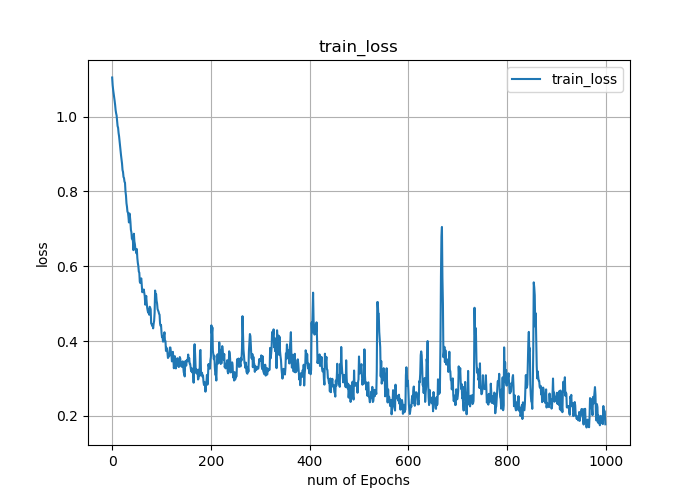
\includegraphics[width=0.7\textwidth]{images/wo_streu.png}
	\caption{Abbildung der Fehlerrate des neuronalen Netzes mit Filterung der Datenpunkte}	\label{fig:wo_streu}
\end{figure}

\subsection{Datensatz ohne Filterung der Datenpunkte}
\begin{figure}[H]
	\centering
		%[natürliche Breite in Pixeln, natürliche Höhe in Pixeln, Abhängigkeit von der Textbreite]
		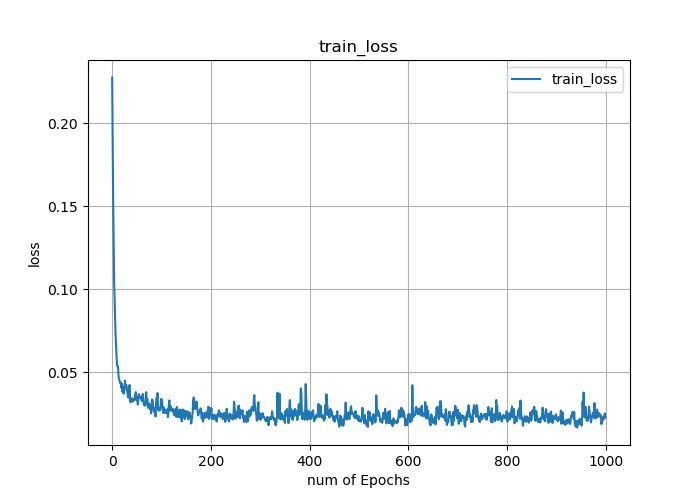
\includegraphics[width=0.7\textwidth]{images/w_streu_nn.png}
	\caption{Abbildung der Fehlerrate des neuronalen Netzes mit allen Datenpunkten}
	\label{fig:w_streu}
\end{figure}

Werden alle Datenpunkte in den Datensätzen gelassen, so liegt die Fehlerrate bei 0,03. Somit klassifiziert das neuronale Netz zu 99,7\% richtig. Damit ist es schon sehr nah an den 100\% und kann schon fast in den Prototypen mit eingebunden werden.

\section{Zusammenfassung der Evaluation}
Aus den vorherigen Kapiteln der Evaluation wird gezeigt, wie verschiedene Probanden mit dem Prototypen umgehen. So ist also nochmal zu sagen, dass der Prototyp durch ersetzen der Ultrasonic-Sensoren eine bessere Möglichkeit bietet um zu erkennen, wann ein Nutzer die Rückenlehne des Sofas verwendet. Wenn diese Sensoren ersetzt werden, kann die Rückenlehne des Sofas auch besser mit in die Verwaltung der Interaktionen einfliessen. 
\newline
\newline
Aus \ref{subsec:ergeb} ist zu erkennen, dass es besser ist ein neuronales Netz mit Daten zu trainieren, die so nah wie möglich an der Realität sind. Zudem verläuft das Training ohne die gefilterten Daten wesentlich besser ab. Es ist nicht wichtig wie viele Daten benutzt werden, sondern wie viele verschiedene Kombinationen dem neuronalen Netz zum trainieren gegeben wird. Durch die geringere Anzahl an Interaktionen die der Datensatz mit Filterung der Datenpunkte vorgibt, ist die Fehlerrate auch dementsprechend höher.

\section{Erkenntnisse aus der Evaluation zum Prototypen}
Aus folgender Überlegung aus dem Kapitel \ref{sub:real}, dass Probanden nach einer Zeit wiederholt die gleiche Sitzposition einnehmen, werden in diesem Kapitel die Schlüsse und Erkenntnisse daraus gezogen. Diese Erkenntnisse sind so beschrieben, dass bestimmte Punkte die Erkenntnis aus der Evaluation bilden.
\newline
So deuten diese Ergebnisse darauf hin, dass es von Vorteil ist, mehr Sensoren zur Erkennung der Interaktionen auf dem Sofa zu verbauen. So können weitere Werte aus den Realwerten gemessen werden, um so noch besser die Interaktionen im neuronalen Netz vorhersagen zu können. Als weitere Möglichkeit geht daraus hervor, nur FSR-Sensoren zu verwenden. Alternativ können auch Sensoren verwendet werden, welche die komplette Fläche einnehmen. Da die Probanden durch ihre Interaktionen auf dem Sofa Druck auf die Oberflächen ausüben, ist dies ein weiterer Grund nur FSR-Sensoren zu benutzen. Zusammengefasst kann also erwähnt werden, dass der Prototyp im aktuellen Zustand noch überarbeitet werden muss, da die Sensoren wie der Ultrasonic-Sensor für die Erkennung nicht von Vorteil ist. Also ist eine weitere Erkenntnis aus der Evaluation, dass für einen Prototypen mit dem Interaktionen aus Sitz- und Liegepositionen erfasst werden, Sensoren zu verwenden, welche ausschließlich den Druck oder die Kraft messen.
\newpage
Anhand des letzten Kapitels wird gezeigt wie Vorhersagen ausfallen, wenn ein Datensatz mit allen Datenpunkten verwendet wird. Zusätzlich wird der Datensatz aus den Sensorwerten erstellt bei dem die Position nur einmal gespeichert wird. Zusammengefasst liegt die Fehlerrate bei dem Datensatz mit den gefilterten Datenpunkten bei 0,16. Dies ist im Vergleich zur Fehlerrate von 0,03 eine großer Unterschied. Dies zeigt, dass das Trainieren mit allen Datenpunkten besser ist. 

